\documentclass[12pt,aspectratio=169]{beamer}
\usepackage{pxfonts}

\usepackage{fancyvrb}
\fvset{%frame=single,
commandchars=\\\{\},
%framesep=1mm,
fontfamily=helvetica,
fontsize=\normalsize
}
%\usepackage[bitstream-charter]{mathdesign}
\usepackage{listings}
\lstset{commentstyle=\color{orange}, keywordstyle=\color{yellow} }

\usepackage{newpxtext}
\usepackage[utf8]{eulerpx}

\usetheme{Boadilla}
\useoutertheme{split}
\usecolortheme{albatross}


\setbeamertemplate{blocks}[rounded][shadow=false]
\setbeamertemplate{navigation symbols}{}
\beamerdefaultoverlayspecification{<+->}


\setbeamercolor*{structure}{fg=green!75!black,bg=blue!70!white}
\setbeamercolor*{normal text}{fg=green!65!black,bg=blue!80!black}
\setbeamercolor{palette primary}{use={structure,normal text},fg=green,bg=structure.bg!75!black}
\setbeamercolor{palette secondary}{use={structure,normal text},fg=structure.fg,bg=structure.bg!60!black}
\setbeamercolor{palette tertiary}{use={structure,normal text},fg=structure.fg,bg=structure.bg!45!black}
\setbeamercolor{palette quaternary}{use={structure,normal text},fg=green,bg=structure.bg!75!black}
\setbeamercolor*{example text}{fg=green!65!black}
\setbeamercolor*{block body}{bg=structure.bg!90!black}
\setbeamercolor*{block body alerted}{bg=structure.bg!90!black}
\setbeamercolor*{block body example}{bg=structure.bg!90!black}
\setbeamercolor*{block title}{parent=structure,bg=structure.bg!75!black}
\setbeamercolor*{block title alerted}{use={structure,alerted text},fg=alerted text.fg!75!structure.fg,bg=structure.bg!75!black}
\setbeamertemplate{navigation symbols}{}
\setbeamertemplate{items}[square]
\setbeamercolor{item projected}{fg=white}
\setbeamercolor*{normal text}{fg=white!90!blue,bg=blue!70!black}
\setbeamercolor*{separation line}{}
\setbeamercolor*{fine separation line}{}
\setbeamercolor{alerted text}{fg=green}

\usepackage[italian]{babel}
\usepackage[utf8]{inputenc}
\usepackage{pgf}
\usepackage{verbatim}
\usepackage{inconsolata}
\usepackage{listings}
\lstset{language=C, frame=single,
  basicstyle=\ttfamily,
  numbers=left, numberstyle=\tiny\color{gray},
  numbersep=5pt, fancyvrb=true
}

\usefonttheme{professionalfonts} % using non standard fonts for beamer
\usefonttheme{serif} % default family is serif
% \usepackage{fontspec}
% \setmainfont{Palatino}

\usepackage{pgf}
\usepackage{tikz}
\usepackage{graphicx}
\usetikzlibrary{%
  arrows,
  arrows.meta,
  positioning,
  calc,
  backgrounds,
  chains,
  matrix,
  patterns,
  automata,
  fit,
  graphs,
  decorations,
  decorations.pathmorphing,
  decorations.pathreplacing,
  decorations.markings,
}

\usepgflibrary{shapes,shapes.geometric}


\usepackage{url}
\usepackage{xmpmulti}
% \usepackage{euler}
%\usepackage[T1]{fontenc}
\pdfpagebox5
% \immediate\write18{sh ./vc}
% \input{vc}

\author{Gianluca Della Vedova}
\title{Elementi di Bioinformatica}
\institute{Univ. Milano--Bicocca\\
  \texttt{https://gianluca.dellavedova.org}}
\date{\today}
%\pgfdeclareimage[height=1cm]{university-logo}{logounimib}
%\logo{\pgfuseimage{university-logo}}


\begin{document}

\begin{frame}
  \titlepage
\end{frame}


\begin{frame}[fragile]
\frametitle{Trie}
\begin{columns}
\begin{column}{0.6\textwidth}
\begin{block}{Trie}
\begin{itemize}
\item
Albero
\item
Query: parola $\in$ dizionario
\item
archi etichettati
\item
Percorso radice-foglia = parola
\end{itemize}
\end{block}
\begin{block}{Dizionario}
ABRACADABRA\\
ARRAY\\
\uncover<3->{\alert{ABRA}}
\end{block}
\end{column}
\begin{column}{0.4\textwidth}
\begin{center}
\onslide<2->{\includegraphics[width=0.5\textwidth]{figures/trie1}}
%\onslide<4->{\includegraphics[width=\textwidth]{figures/trie3}}
\end{center}
\end{column}
\end{columns}
\end{frame}

\begin{frame}[fragile]
\frametitle{Trie}
\begin{columns}
\begin{column}{0.6\textwidth}
\begin{block}{Terminatore}
\$ non appartiene all'alfabeto
\end{block}
\onslide<2->{\begin{block}{Dizionario}
ABRACADABRA\$\\
ARRAY\$\\
ABRA\$
\end{block}}
\end{column}
\begin{column}{0.4\textwidth}
\begin{center}
\onslide<3->{\includegraphics[width=0.8\textwidth]{figures/trie4}}
\end{center}
\end{column}
\end{columns}
\end{frame}

\begin{frame}[fragile]
\frametitle{Suffix tree}
\begin{columns}
\begin{column}{0.5\textwidth}
\begin{block}{Definizione}
\begin{itemize}[<+->]
% \item
% Testo $T$
\item
Trie compatto di tutti i suffissi di $T\$$
\item
Le etichette degli archi uscenti da $x$ iniziano con simboli diversi
\item
suffissi $\Leftrightarrow$ percorso radice-foglia
\end{itemize}
\end{block}
\end{column}
\begin{column}{0.5\textwidth}
\begin{center}
\uncover<4->{\includegraphics[width=\textwidth]{figures/Suffix_tree_BANANA}

BANANA\$}
\end{center}
\end{column}
\end{columns}
\end{frame}

\begin{frame}[fragile]
\frametitle{Suffix tree 2: Definizione}
\begin{itemize}
\item
foglie etichettata con posizione inizio suffisso
\item
path-label$(x)$: concatenazione etichette
\item
string-depth$(x)$: lunghezza path-label$(x)$
\item
Pattern matching = visita
\end{itemize}
\begin{block}{Problemi}
\begin{itemize}[<+->]
\item
Spazio $O(n^{2})$
\item
Puntatori al testo (posizioni)
\item
Spazio $20n$ bytes
\end{itemize}
\end{block}
\end{frame}

\begin{frame}[fragile]
\frametitle{Suffix array}
\begin{block}{Definizione}
\begin{itemize}[<+->]
\item
Array dei suffissi in ordine lessicografico
\item
Posizioni iniziali del suffisso nell'array
\item
Spazio $4n$ bytes
\item
$Lcp[i]$: lunghezza prefisso comune $SA[i]$, $SA[i+1]$
\end{itemize}
\end{block}
\uncover<5->{\begin{block}{BANANA\$}
\begin{tabular}[l]{|c|l|l|l|l|l|l|l|}
\hline
$i$&1&2&3&4&5&6&7\\
$SA$&7&6&4&2&1&5&3\\
$Lcp$&0&1&3&0&0&2&-\\\hline
\end{tabular}}
\end{block}
\end{frame}

\begin{frame}[fragile]
\frametitle{Da Suffix tree a Suffix array}
\begin{columns}
\begin{column}{0.5\textwidth}
\begin{itemize}[<+->]
\item
Visita depth-first di $ST$
\item
archi uscenti di ogni nodo in ordine lessicografico
\item
$Lcp[i]$ = string-depth di $lca(i,i+1)$
\end{itemize}
\end{column}
\begin{column}{0.4\textwidth}
\begin{center}
\onslide<1->{\includegraphics[width=\textwidth]{figures/Suffix_tree_BANANA}}
%\onslide<4->{\includegraphics[width=\textwidth]{figures/trie3}}
\end{center}
\end{column}
\end{columns}
\end{frame}

\begin{frame}[fragile]
\frametitle{Da Suffix array a Suffix tree}
\begin{columns}
\begin{column}{0.5\textwidth}
\begin{itemize}[<+->]
\item
$Lcp = 0$:  partizione $SA$
\item
corrispondono ai figli della radice
\item
ricorsione prendendo i numeri minimi
\end{itemize}
\begin{block}{BANANA\$}
\begin{tabular}[l]{|c|l|l|l|l|l|l|l|}
\hline
$i$&0&1&2&3&4&5&6\\
$SA$&7&6&4&2&1&5&3\\
$Lcp$&0&1&3&0&0&2&-\\\hline
\end{tabular}
\end{block}
\end{column}
\begin{column}{0.5\textwidth}
\begin{center}
\only<2>{\includegraphics[width=\textwidth]{figures/Suffix_tree_BANANA-level1}}
\only<3>{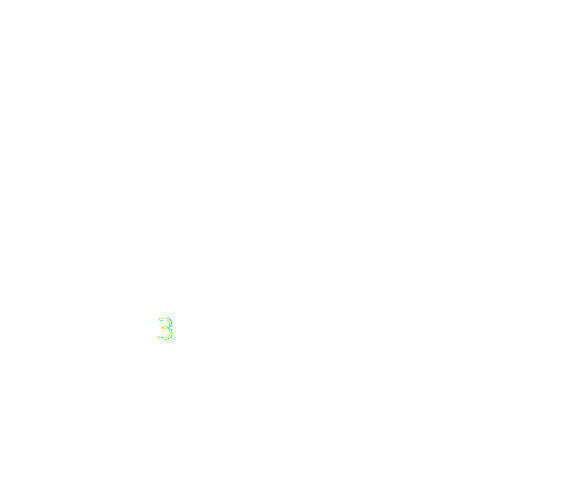
\includegraphics[width=\textwidth]{figures/Suffix_tree_BANANA-level2}}
\only<4>{\includegraphics[width=\textwidth]{figures/Suffix_tree_BANANA-level3}}
\only<5>{\includegraphics[width=\textwidth]{figures/Suffix_tree_BANANA}}
\end{center}
\end{column}
\end{columns}
\end{frame}



\begin{frame}
\frametitle{Suffix tree generalizzato}
\begin{columns}
\begin{column}{0.8\textwidth}
\begin{center}
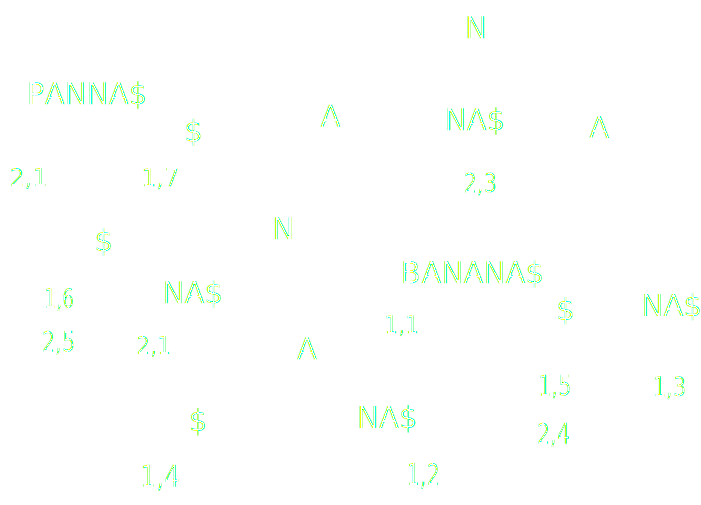
\includegraphics[width=0.8\textwidth]{figures/ST-banana-panna}
\end{center}
\end{column}
\begin{column}{0.18\textwidth}
$s_{1}$: BANANA\$\\
$s_{2}$: PANNA\$
\end{column}
\end{columns}
\end{frame}


\begin{frame}[fragile]
\frametitle{Sottostringa comune più lunga di due stringhe}
\begin{block}{Due stringhe $s_{1}$ e $s_{2}$}
\begin{itemize}[<+->]
\item
Suffix tree generalizzato = insieme di stringhe
\item
$ST(s_{1}\$_{1}s_{2}\$_{2})$
\item
Nodo $x$ con foglie di $s_{1}$ e $s_{2}$
\item
Sottostringa di $s_{1}$ e $s_{2}$
\item
$ST(s_{1}\$s_{2}\$)$
\item
Max string-depth
\end{itemize}
\end{block}
\end{frame}



\begin{frame}[containsverbatim]\frametitle{Licenza d'uso}
  \small

  Quest'opera {\`e} soggetta alla licenza Creative Commons:
Attribuzione-Condividi allo stesso modo 4.0.
  (\verb+https://creativecommons.org/licenses/by-sa/4.0/+).

Sei libero di riprodurre, distribuire, comunicare al pubblico, esporre
in pubblico, rappresentare, eseguire, recitare e modificare quest'opera
alle seguenti condizioni:
\begin{itemize}
\item
Attribuzione — Devi attribuire la paternit{\`a} dell'opera nei modi
indicati dall'autore o da chi ti ha dato l'opera in licenza e in modo tale da
non suggerire che essi avallino te o il modo in cui tu usi l'opera.
\item
Condividi allo stesso modo — Se alteri o trasformi quest'opera, o se
la usi per crearne un'altra, puoi distribuire l'opera risultante solo con
una licenza identica o equivalente a  questa.
\end{itemize}
%  \vspace*{1cm}
\end{frame}

\end{document}
